%%%%%%%%%%%%%%%%%%%%%%%%%%%%%%%%%%%%%%%%%
%
% CMPT 435
% Fall 2022
% Assignment 3
%
%%%%%%%%%%%%%%%%%%%%%%%%%%%%%%%%%%%%%%%%%

%%%%%%%%%%%%%%%%%%%%%%%%%%%%%%%%%%%%%%%%%
% Short Sectioned Assignment
% LaTeX Template
% Version 1.0 (5/5/12)
%
% This template has been downloaded from: http://www.LaTeXTemplates.com
% Original author: % Frits Wenneker (http://www.howtotex.com)
% License: CC BY-NC-SA 3.0 (http://creativecommons.org/licenses/by-nc-sa/3.0/)
% Modified by Alan G. Labouseur  - alan@labouseur.com
%
%%%%%%%%%%%%%%%%%%%%%%%%%%%%%%%%%%%%%%%%%

%----------------------------------------------------------------------------------------
%	PACKAGES AND OTHER DOCUMENT CONFIGURATIONS
%----------------------------------------------------------------------------------------

\documentclass[letterpaper, 10pt,DIV=13]{scrartcl} 

\usepackage[T1]{fontenc} % Use 8-bit encoding that has 256 glyphs
\usepackage[english]{babel} % English language/hyphenation
\usepackage{amsmath,amsfonts,amsthm,xfrac} % Math packages
\usepackage{sectsty} % Allows customizing section commands
\usepackage{graphicx}
\usepackage{algorithm, algpseudocode}
\usepackage{listings}
\usepackage{parskip}
\usepackage{lastpage}
\usepackage{color}
\usepackage{qtree}
\usepackage{xcolor}
\usepackage{colortbl}

\allsectionsfont{\normalfont\scshape} % Make all section titles in default font and small caps.

\usepackage{fancyhdr} % Custom headers and footers
\pagestyle{fancyplain} % Makes all pages in the document conform to the custom headers and footers

\fancyhead{} % No page header - if you want one, create it in the same way as the footers below
\fancyfoot[L]{} % Empty left footer
\fancyfoot[C]{} % Empty center footer
\fancyfoot[R]{page \thepage\ of \pageref{LastPage}} % Page numbering for right footer

\renewcommand{\headrulewidth}{0pt} % Remove header underlines
\renewcommand{\footrulewidth}{0pt} % Remove footer underlines
\setlength{\headheight}{13.6pt} % Customize the height of the header

\numberwithin{equation}{section} % Number equations within sections (i.e. 1.1, 1.2, 2.1, 2.2 instead of 1, 2, 3, 4)
\numberwithin{figure}{section} % Number figures within sections (i.e. 1.1, 1.2, 2.1, 2.2 instead of 1, 2, 3, 4)
\numberwithin{table}{section} % Number tables within sections (i.e. 1.1, 1.2, 2.1, 2.2 instead of 1, 2, 3, 4)

\setlength\parindent{0pt} % Removes all indentation from paragraphs.

\binoppenalty=3000
\relpenalty=3000

\algrenewcommand{\algorithmiccomment}[1]{\hskip1em\textit{$//$ #1}}

%----------------------------------------------------------------------------------------
%	TITLE SECTION
%----------------------------------------------------------------------------------------

\newcommand{\horrule}[1]{\rule{\linewidth}{#1}} % Create horizontal rule command with 1 argument of height

\title{	
   \normalfont \normalsize 
   \textsc{CMPT 435 - Fall 2022 - Dr. Labouseur} \\[10pt] % Header stuff.
   \horrule{0.5pt} \\[0.25cm] 	% Top horizontal rule
   \huge Assignment Three  \\     	    % Assignment title
   \horrule{0.5pt} \\[0.25cm] 	% Bottom horizontal rule
}

\author{Josh Seligman \\ \normalsize joshua.seligman1@marist.edu}

\date{\normalsize\today} 	% Today's date.

\begin{document}
\maketitle % Print the title

\section{Linear Search}
\subsection{The Algorithm}\label{linearSearch}
Linear search is a searching algorithm that walks through an array and continues on until either it finds the target element or reaches the end of the array. As shown in Algorithm \ref{algorithm:linearSearch}, the function has to compare the target value with every element in the array until the condition in the while loop becomes false. Since the entire array is being searched, no assumptions have to be made about the initial status of the array, which means that the array does not have to be sorted or in any particular order prior to running the search.

\begin{algorithm}
  \caption{Linear Search Algorithm}
  \label{algorithm:linearSearch}
  %Documentation for algorithmicx: https://texdoc.org/serve/algorithmicx/0
  \begin{algorithmic}[1]
      \Procedure{LinearSearch}{$arr$, $target$}
        \State $i \gets 0$ \Comment{Start at the beginning of the array}
        \While{$i~<~len(arr)~\&\&~arr[i]~!=~target$} \Comment{Search through the entire array or until the target is found}
          \State $i++$
        \EndWhile
        \If{$i == len(arr)$}
          \State $i = -1$ \Comment{Set $i$ to -1 to note that the target is not in the array}
        \EndIf
        \State \Return $i$
      \EndProcedure
  \end{algorithmic}
\end{algorithm}

\subsection{Asymptotic Analysis and Comparisons}
As mentioned in Section \ref{linearSearch}, performing a linear search requires going through each element until the target is found or until the end of the array is reached. The performance of linear search varies drastically on the position of the target element relative to the front of the array. For instance, linear search will be really fast when the target is near the front as the algorithm terminates upon finding the element. However, if the target is near the end of the array, the algorithm will have to iterate through nearly the entire array. Thus, for a randomly sorted list, the average expected case will be $\frac{n}{2}$ iterations. Also, at the worst case, the number of iterations will be equal to the number of elements in the array. Therefore, as its name implies, linear search runs in linear time $O(n)$. Table \ref{comparisonsTable} shows the average number of comparisons made for 42 of the 666 magic items, which for the case of linear search, was 341.67. This lines up with the expected case for the searching algorithm of $\frac{n}{2}$ as, for a list of 666 items, about 333 will have to be searched and compared with before the target value is found.

\section{Binary Search}
\subsection{The Algorithm}\label{binarySearch}
Binary search is a searching algorithm that takes an already sorted list and progressively cuts it in half until there is only 1 element left, which is the one that is being searched for. As shown in Algorithm \ref{algorithm:binarySearch}, each recursive call on lines 8 and 10 makes the problem smaller by moving the start or stop limits to a single side of the midpoint, which effectively cuts the array in half at each level of the recursion tree. Also, Figure \ref{figure:binarySearch} illustrates how binary search divides the array in half to eventually find the target element.

\begin{algorithm}
  \caption{Binary Search Algorithm}
  \label{algorithm:binarySearch}
  %Documentation for algorithmicx: https://texdoc.org/serve/algorithmicx/0
  \begin{algorithmic}[1]
      \Procedure{BinarySearch}{$arr$, $target$, $start$, $stop$}
        \State $out \gets -1$ \Comment{Assume the element is not found, by setting the default output to -1}
        \If{start <= stop} \Comment{Working in a valid range}
          \State $mid \gets \lfloor\frac{(start + stop)}{2}\rfloor$ \Comment{Get the middle of the range}
          \If{$target == arr[mid]$}
            \State $out \gets mid$ \Comment{Target found at position $mid$}
          \ElsIf{$target < arr[mid]$} \Comment{Target is in bottom half of the array}
            \State $out \gets BinarySearch(arr, target, start, mid - 1)$ \Comment{Do binary search on lower half of array}
          \Else \Comment{Target is in top half of the array}
            \State $out \gets BinarySearch(arr, target, mid + 1, stop)$ \Comment{Do binary search on top half of array}
          \EndIf
        \EndIf
        \State \Return $out$
      \EndProcedure
  \end{algorithmic}
\end{algorithm}

\begin{center}
  \begin{tabular}{|c|c|c|c|c|c|c|c|c|c|}
    % Documentation for coloring the cells of a table: https://mirror.math.princeton.edu/pub/CTAN/macros/latex/contrib/colortbl/colortbl.pdf
    \hline
    \rowcolor{blue!20}0 & 1 & 2 & 3 & 4 & 5 & 6 & 7 & 8 & 9 \\
    \hline
    0 & 1 & 2 & 3 & 4 & \cellcolor{blue!20}5 & \cellcolor{blue!20}6 & \cellcolor{blue!20}7 & \cellcolor{blue!20}8 & \cellcolor{blue!20}9 \\
    \hline
    0 & 1 & 2 & 3 & 4 & \cellcolor{blue!20}5 & \cellcolor{blue!20}6 & 7 & 8 & 9 \\
    \hline
    0 & 1 & 2 & 3 & 4 & 5 & \cellcolor{blue!20}6 & 7 & 8 & 9 \\
    \hline
  \end{tabular}
\captionof{figure}{A visualization of the binary search algorithm. The blue shaded areas are the parts of the array being considered at each step of the recursion tree until there is only the target element left.}
\label{figure:binarySearch}
\end{center}

\subsection{Asymptotic Analysis and Comparisons}
Binary search, similar to merge sort and quicksort, divides the array in half at each step of the recursion tree. This makes the recurrence relation of binary search to be $T(n) = T(\frac{n}{2}) + C$, where $T(\frac{n}{2})$ is the time to perform binary search on the half of the array and $C$ is the constant time to perform the comparisons. Thus, since the array is being divided in half until the size of the array being considered is 1, the number of times binary search will be recursively called at worst case will be $log_2n$ times, which makes it run in $O(log_2n)$ time.

$O(log_2n)$ is a huge improvement over $O(n)$ for linear search. However, the one tradeoff is that binary search needs to have an already sorted array. Thus, if the array is not sorted, an additional $n * log_2n$ time will need to be added to put the array in a state to use binary search. Therefore, linear search may be the better option for one and done search operations, but binary search with a sort will catch up as the number of search operations increases. The mathematical equation to determine this point is $x * n > x * log_2n + n * log_2n$, where $x$ is the number of searching operations that have to be done on the unsorted array. For an array of 666 sorted items, binary search required an avereage of 8.57 comparisons to retrieve 42 random items, which is around $n * log_2n = 9.37$, or the number of levels in the recursion tree.

\subsection{Hashing with Chaining}
A hash table is a data structure that stores data in an array and uses a hash function to determine the position in the array to store the data. Hash tables have 2 main functions: get and put, and both of these are provided in Algorithms \ref{algorithm:hashGet} and \ref{algorithm:hashPut}, respectively. Since an array has a fixed size, there are 2 initial problems with hash tables. The first is that the output of a hash function may not be directly translatable to an array index. As displayed on line 19 of Listing \ref{lst:hashFunc}, once the sum of the ordinal codes is calculated, modulus division is performed to get the hash code to be on the range $[0, size - 1]$, which are all valid indices within the array. The other issue is caused when 2 different elements return the same hash code, which is called a collision. A hash table may implement a method called probing by searching for an empty space within the array to put the value, but is restricted by the size of the created array. Chaining is the other way to resolve this problem of duplicate hash codes. Rather than searching for an empty spot in the array, chaining stares a linked list at each element in the array, and the value that is being put into the hash table can be added to the linked list at the index generated by the hash function. Additionally, unlike probing, chaining is not limited to the size of the array being used as a linked list is only limited by the size of memory. See Figure \ref{figure:hashing} for a visual understanding of hashing with chaining.

\begin{algorithm}
  \caption{Hash Table Get Function}
  \label{algorithm:hashGet}
  %Documentation for algorithmicx: https://texdoc.org/serve/algorithmicx/0
  \begin{algorithmic}[1]
      \Procedure{Get}{$value$}
        \State $hashCode \gets hash(value)$ \Comment{Generate the hash code for the value}
        \State $cur \gets table[hashCode]$ \Comment{Start iterating at the head of the linked list at the index the hash function returned}
        \State $found = false$ \Comment{Assume the vaule is not found}
        \While{$!found~\&\&~cur~!= null$}
          \If{$cur.data == value$}
            \State $found = true$ \Comment{The value was found}
          \EndIf
          \State $cur = cur.next$ \Comment {Move to the next element in the linked list}
        \EndWhile
        \State \Return $found$
      \EndProcedure
  \end{algorithmic}
\end{algorithm}

\begin{algorithm}
  \caption{Hash Table Put Function}
  \label{algorithm:hashPut}
  %Documentation for algorithmicx: https://texdoc.org/serve/algorithmicx/0
  \begin{algorithmic}[1]
      \Procedure{Put}{$value$}
        \State $hashCode \gets hash(value)$ \Comment{Generate the hash code for the value}
        \State $curHead \gets table[hashCode]$ \Comment{Going to work with the head of the list}
        \State $newHead = new Node(value)$ \Comment{Create the new node}
        \If {$curHead~!= null$}
          \State $newHead.next = curHead$ \Comment{Place the new node ahead of the current head}
        \EndIf
        \State $table[hashCode] = newHead$ \Comment{Update the table entry to point to the new head}
      \EndProcedure
  \end{algorithmic}
\end{algorithm}

\begin{figure}[ht] 
  \centering 
  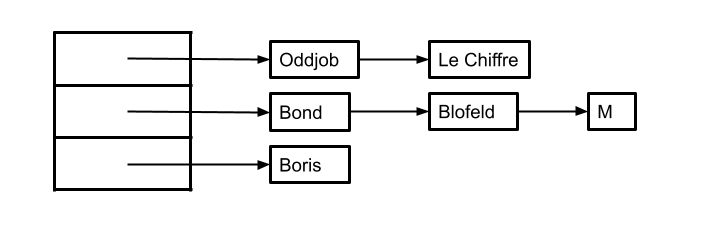
\includegraphics[width=15cm]{hashing}
  \caption{Example hash table of James Bond characters that uses chaining. The hash function used is the number of characters (excluding spaces) mod the size of the array.}
  \label{figure:hashing}
\end{figure}

\subsection{Asymptotic Analysis and Comparisons}
The functions of a hash table are extremely efficient and do not completely rely on the number of elements stored in the hash table. First, the get function for a hash table computes the hash code, which is just a mathematical formula, and then accesses the element based on the output of the hash function. However, depending on the method being used for collisions, the time to access the element varies. This variation is called the load factor and can be noted with $\alpha$. In the case of chaining, as described in Algorithm \ref{algorithm:hashGet} and demonstrated in Listing \ref{lst:hashGet} on lines 16-29, the linked list stored at the index of the array has to be iterated over. Assuming the hash function produces evenly distributed hash codes, the number of elements that have to be iterated through will on average be $\frac{n}{size~of~array}$, which is the value for $\alpha$. Therefore, the runtime for the hash table get function is $O(1) + \alpha$. Table \ref{comparisonsTable} also highlights the average number of comparisons needed for performing the hash table get function. For a random selection of 42 of the 666 magic items, it took an average of 3.19 comparisons to retrieve the item, which is a drastic improvement over both binary search and linear search.

The C++ implementation for the put function for hash tables is shown in Listing \ref{lst:hashPut} and is a bit simpler compared to the get function. After computing the hash code on line 3, the put function creates a new node and inserts it at the front of the list. Just like a stack, since the front of the list is being used, there is no need to traverse through the entire list. Therefore, the put function runs in constant time $O(1)$.

\section{Appendix}
\subsection{Comparisons Table}\label{comparisonsTable}
\begin{center}
  \begin{tabular}{|c|c|}
    \hline
    Search Name & Comparisons \\
    \hline
    Linear Search & 341.67 \\
    \hline
    Binary Search & 8.57 \\
    \hline
    Hashing & 3.19 \\
    \hline
  \end{tabular}
\captionof{table}{A table of the number of comparisons made and time to get an item from an array or hash table.}
\end{center}

\lstset{numbers=left, numberstyle=\tiny, stepnumber=1, numbersep=5pt}

% Colors and lstset for syntax highlighting from https://www.overleaf.com/latex/examples/syntax-highlighting-in-latex-with-the-listings-package/jxnppmxxvsvk
\definecolor{mygreen}{rgb}{0,0.6,0}
\definecolor{mygray}{rgb}{0.5,0.5,0.5}
\definecolor{mymauve}{rgb}{0.58,0,0.82}
\lstset{
  backgroundcolor=\color{white},   % choose the background color
  basicstyle=\footnotesize,        % size of fonts used for the code
  breaklines=true,                 % automatic line breaking only at whitespace
  captionpos=b,                    % sets the caption-position to bottom
  commentstyle=\color{mygreen},    % comment style
  escapeinside={\%*}{*},          % if you want to add LaTeX within your code
  keywordstyle=\color{blue},       % keyword style
  stringstyle=\color{mymauve},     % string literal style
}

\subsection{Linear Search}
\lstinputlisting[caption = Linear Search (C++), label = lst:linearSearch, language = C++, firstline = 6, lastline = 30, firstnumber = 1]{./../searches.cpp}

\subsection{Binary Search}
\lstinputlisting[caption = Binary Search (C++), label = lst:binarySerach, language = C++, firstline = 32, lastline = 67, firstnumber = 1]{./../searches.cpp}

\subsection{Hashing with Chaining}
\lstinputlisting[caption = Simple Hash Function, label = lst:hashFunc, language = C++, firstline = 86, lastline = 106]{./../hashTable.cpp}
\lstinputlisting[caption = Hash Table Get with Chaining, label = lst:hashGet, language = C++, firstline = 37, lastline = 67]{./../hashTable.cpp}
\lstinputlisting[caption = Hash Table Put with Chaining, label = lst:hashPut, language = C++, firstline = 69, lastline = 84]{./../hashTable.cpp}

\end{document}